\documentclass{article}
\usepackage{graphicx}
\graphicspath{ {./images/} }
\usepackage[export]{adjustbox}
\usepackage{amsmath}


\title{I-iespēja: 1. mājasdarbs}
\author{Gunārs Ābeltiņš}
\date{2022-10-16}

\begin{document}

\maketitle

Ir iespējams izvēlēties 7 vektorus no regulāra 12 stūra, lai to summa būtu nulles vektors. 

Ja vajadzētu izvēleties para skaitli vektorus, tad varetu ņemt pa pāriem pretejos vektorus, jo daudzstūris ir simetriskas formas, tāpēc, ja vektori ir preteji, tad to summa būs nulles vektors.

Ir iespējams arī izvēleties 3 vektorus, lai to summa būtu nulles vektors, jo katrs stūris ir 150 grādi (10 * 100 / 12 = 150) tāpēc, ja pa apli paņem katru ceturto malu, tad to summa būs nulles vektors. Tas ir leņķis starp malām, kas ir blakus bus 150. Ja viena pa vidu, tad 120. Ja divas, tad 90. Ja trīs, tad 60.

Tātad var paņemt divus pārus ar pretējiem vektoriem un vienu regulāru trijsūri (2+2+3=7), lai to summa būtu nulles vektors.

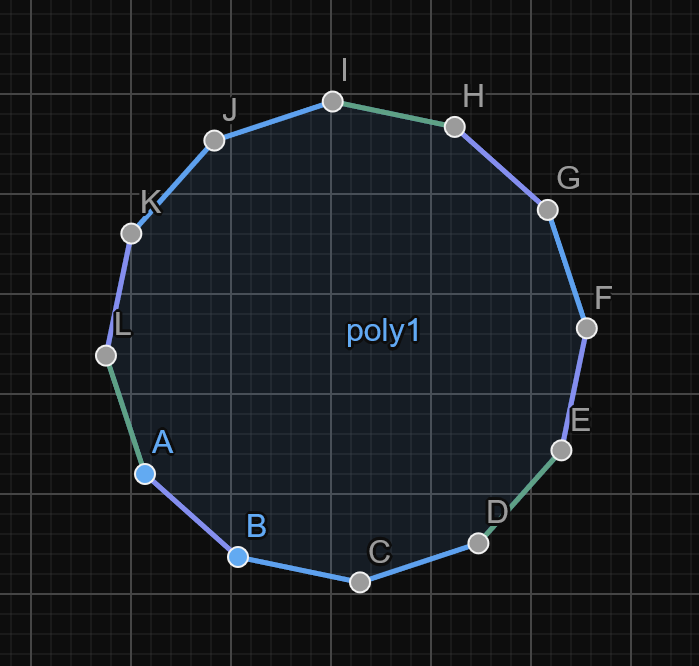
\includegraphics[width=0.5\textwidth, center]{polygon.png}

Ilustrācija pretējie vektori ir violēti un regulārs trijstūris ir zaļš.

\end{document}